\let\negmedspace\undefined
\let\negthickspace\undefined
\documentclass[journal]{IEEEtran}
\usepackage[a5paper, margin=10mm, onecolumn]{geometry}
%\usepackage{lmodern} % Ensure lmodern is loaded for pdflatex
\usepackage{tfrupee} % Include tfrupee package

\setlength{\headheight}{1cm} % Set the height of the header box
\setlength{\headsep}{0mm}     % Set the distance between the header box and the top of the text

\usepackage{gvv-book}
\usepackage{gvv}
\usepackage{cite}
\usepackage{amsmath,amssymb,amsfonts,amsthm}
\usepackage{algorithmic}
\usepackage{graphicx}
\usepackage{textcomp}
\usepackage{xcolor}
\usepackage{txfonts}
\usepackage{listings}
\usepackage{enumitem}
\usepackage{mathtools}
\usepackage{gensymb}
\usepackage{comment}
\usepackage[breaklinks=true]{hyperref}
\usepackage{tkz-euclide} 
\usepackage{listings}
% \usepackage{gvv}                                        
\def\inputGnumericTable{}                                 
\usepackage[latin1]{inputenc}                                
\usepackage{color}                                            
\usepackage{array}                                            
\usepackage{longtable}                                       
\usepackage{calc}                                             
\usepackage{multirow}                                         
\usepackage{hhline}                                           
\usepackage{ifthen}                                           
\usepackage{lscape}
\begin{document}

\bibliographystyle{IEEEtran}
\vspace{3cm}

\title{1/1.6/20}
\author{EE24BTECH11040 - Mandara Hosur}
% \maketitle
% \newpage
% \bigskip
{\let\newpage\relax\maketitle}

\renewcommand{\thefigure}{\theenumi}
\renewcommand{\thetable}{\theenumi}
\setlength{\intextsep}{10pt} % Space between text and floats


\numberwithin{equation}{enumi}
\numberwithin{figure}{enumi}
\renewcommand{\thetable}{\theenumi}


\textbf{Question:}\\
Show that the points $\brak{-2,3,5}$, $\brak{1,2,3}$ and $\brak{7,0,-1}$ are collinear.
\\
\textbf{Solution:}\begin{table}[h!]    
  \centering
  \begin{tabular}[12pt]{ |c| c|}
    \hline
    \textbf{Given Points} & \textbf{Description} \\ 
    \hline
    $\brak{-2,3,5}$ & Point $\vec{A}$ \\
    \hline 
    $\brak{1,2,3}$ & Point $\vec{B}$\\
    \hline
    $\brak{7,0,-1}$ & Point $\vec{C}$\\
    \hline 
    \end{tabular}

  \caption{Given Information}
  \label{Table 1}
\end{table} \\

The matrix 
\begin{align}
\myvec{\vec{B}-\vec{A} & \vec{C}-\vec{A}}^\top = \myvec{3 & -1 & -2 \\ 
                                                        9 & -3 & -6} \\
      \xleftrightarrow[]{R_2 = R_2 - 3R_1}
	 \myvec{3 & -1 & -2 \\ 0 & 0 & 0}
\end{align}
has rank of 1. \\ \\
Hence, it has been proved that the three given points are collinear. 

\begin{figure}[h]
    \centering
    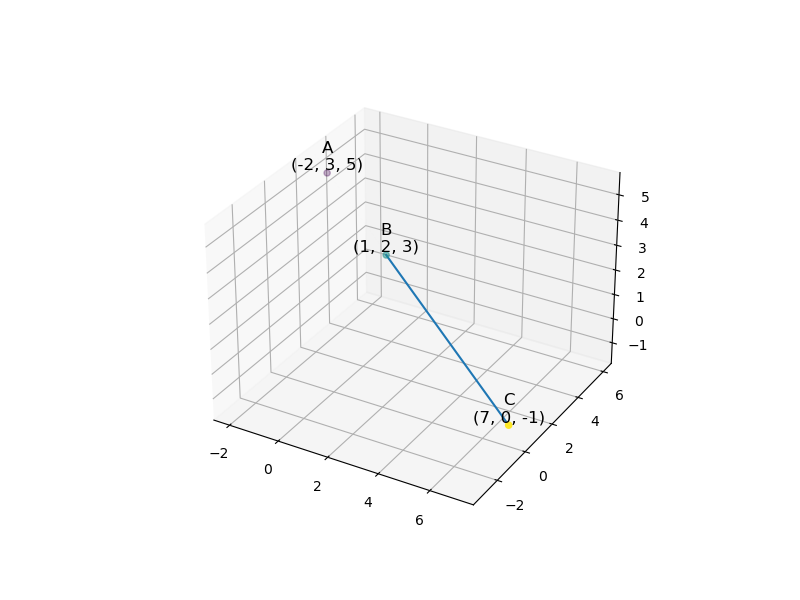
\includegraphics[width=\columnwidth]{figs/fig.png}
    \caption{3D plot of line through points $\vec{A}$, $\vec{B}$, $\vec{C}$}
 \end{figure}

\end{document}
